\documentclass[../skript.tex]{subfiles}


\chapter{The acoustic scattering Problem in full space}\label{c1}

	\section{Introduction}\label{c1se1}

		We study the wave equation in full space $\mathbb{R}^d,\,d\in\{1,2,3\}$.
		\begin{IEEEeqnarray*}{rCl}
			\frac{\partial^2}{\partial t^2}p + \gamma\frac{\partial}{\partial t}p &=& c^2\Delta p
		\end{IEEEeqnarray*}
		Where 
		\begin{IEEEeqnarray*}{rCl}
			c = c(x) && \text{ speed of sound}\\
			\gamma = \gamma(x) && \text{ damping coefficient}
		\end{IEEEeqnarray*}

		Assume \emph{time-periodic behaviour}
		\[
			p(x,t) = Re[ u(x)e^{-i\omega t}]
		\]
		with frequency $\omega$ and a real-valued function $u$.\newline\noindent
		Since 
		\begin{IEEEeqnarray*}{rCl}
			\frac{\partial^2p(x,t)}{\partial t^2} &=& \re [-\omega^2 u(x) e^{-i\omega t}]\\
			\frac{\partial p(x,t)}{\partial t} &=& Re[-i\omega u(x)e^{-i\omega t}] \\
			\Delta p(x,t) &=&\re [\Delta u(x)] e^{-i\omega t}]
		\end{IEEEeqnarray*}
		for all times $t>0$, we infer
		\[
			-\omega^2 u - \gamma i\omega u = c^2 \Delta u,\quad\text{ in }\mathbb{R}^d.
		\]
		This is equivalent to
		\[
			\Delta u + \frac{\omega^2}{c^2}\left(1+\frac{i\gamma}{\omega}\right)u = 0.
		\]
		We assume, that $c = c_0$ is constant in free space (reference value). We can now define a \emph{wave number}
		\[
			\kappa = \overbrace{\underbrace{\frac{\omega}{c_0}}_{>0}}^{>0} > 0
		\] 
		and the \emph{index of refraction}
		\[
			n(x) = \frac{c_0^2}{c(x)^2}\left(1+i\frac{\gamma}{\omega}\right).
		\]
		This results in the \emph{Helmholtz-Equation}
		\[
			\Delta u + \kappa^2nu = 0,\quad\text{ in }\mathbb{R}^d.
		\]
		We assume that there exists $a>0$ such that
		\[
			c(x) = c_0 \text{ and } \gamma(x) = 0,\quad\forall |x|>a,
		\]
		that means inhomogeneities of the medium lie inside some bounded region (inside a ball). Furthermore we assume, that outside this ball of radius $a$, $\overline{B_a(0)}$, there are sources that generate plane waves, that is functions of the type
		\[
			u^{in} (x) = e^{i k x\cdot\hat{\theta}},
		\]
		where $|\hat{\theta}| = 1$ for $\hat{\theta}\in\mathbb{R}^d$ and $\cdot$ denotes the inner product in $\mathbb{R}^d$. Then, $u^{in}$ satisfies
		\[
			\Delta u^{in} + k^2 u^{in} = 0.
		\]
		(just calculation).
		This $u^{in}$ generates a \emph{scattered field} $u^s$. The \emph{total field}
		\[
			u = u^{in} + u^s
		\]
		satisfies 
		\[
			\Delta u + \kappa^2 n u = 0.
		\]
		\begin{figure}\label{c1se1fig1}
			\centering
			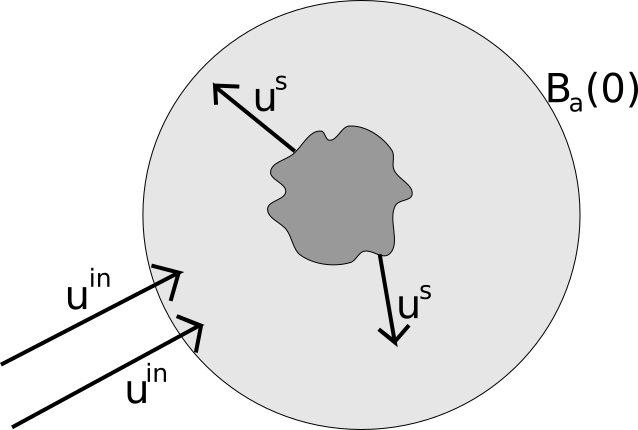
\includegraphics[width=0.5\textwidth]{Images/VL-20-10-2015_1.png}
			\caption{Visualization of the problem}
		\end{figure}

		Furthermore we assume \emph{Sommerfeld's radiation condition} ($r = |x|$):
		\[
			\frac{\partial u^s}{\partial r} - i\kappa u^s(x) = o\left(r^{\frac{1-d}{2}}\right),\quad\text{as } r=|x|\to\infty
		\]
		uniformly in $\frac{x}{|x|}$.

	\section{Theory for the direct Scattering Problem in $\mathbb{R}^3$}\label{c1se2}

		Throughout this section $d=3$ holds! Furthermore 
		\begin{enumerate}
			\item $\hat{\theta}\in\mathbb{R}^3$ with $|\hat{\theta}| = 1$ defines the \emph{indicent field}
				\[
					u^{in}(x) = e^{-i\kappa\hat\theta\cdot x},\quad x\in\mathbb{R}^d
				\]
				\item $\kappa\in\mathbb{R}, \kappa>0$
				\item $n\in L^\infty(\mathbb{R}^3),\re n\geq 0, \im n\geq 0$ and $n(x) = 1$ for all $x\in\mathbb{R}^3\setminus B_a(0)$ and some $a>0$
		\end{enumerate}
		We recall
		\[
			H^1_{loc}(\mathbb{R}^3) \coloneqq \{u:\mathbb{R}^3\to\mathbb{C}:\,u|_K\in H^1(K),\quad\text{for every }K=B_R(0)\text{ and any }R>0\}
		\]
		The \emph{Scattering Problem} reads as follows
		\begin{definition}[Scattering Problem (S)]\label{c1se2prbS}
			Given $\hat\theta,\kappa,n$ as above. Seek $u\in H^1_{loc}(\mathbb{R}^3)$ such that
			\[
				\Delta u + \kappa^2nu = 0
			\]
			in $\mathbb{R}^3$ in the weak sense, that is
			\[
				\int_{\mathbb{R}^3} \left( \nabla u\cdot\nabla\bar{\Psi}-\kappa n u \bar{\Psi} \right)\,dx = 0
			\]
			for any $\Psi\in H^1(\mathbb{R}^3)$ with compact support, and s.t.
			\[
				u^s = u - u^{in}
			\]
			satisfies Sommerfeld's radiation condition ($d=3$, sharper version)
			\[
				\frac{\partial u^s}{\partial r} - i\kappa u^s = O\left(\frac{1}{r^2}\right),\quad\text{uniformly in }\hat x = \frac{x}{|x|} \text { as } r=|x| \to\infty 
			\]
		\end{definition}
		\begin{remark}
			Regularity-theory tells us, that the radiation condition is well-defined, given the assumptions from \cref{c1se2prbS}.
		\end{remark}
		\begin{theorem}[Rellich's Lemma]\label{c1se2thm1}
			Let $u$ satisfy $\Delta u + \kappa^2 u$ for every $|x|>a$. The following property 
			\[
				\lim_{R\to\infty} \int_{|x|=R} |u(x)|^2\,dS = 0
			\]
			implies, that $u(x) = 0$ for all $|x| > a$.
		\end{theorem}
		\begin{remark}
			Vice versa, if the property in \cref{c1se2thm1} does not hold, then $u$ cannot vanish for all $|x| > a$.
		\end{remark}
		\begin{proof}
			Employs spherical Bessel functions, see e.g. 
			%BIBTEX [Colton, Kress].
		\end{proof}
		For the proof of uniqueness, we require results on periodic differential equations. We recall \emph{Fourier representations of periodic functions}:\newline\noindent
		Define
		\[
			Q\coloneqq (-\pi,\pi)^3\subseteq\mathbb{R}^3.
		\]
		The functions
		\[
			\{\varphi_j: j\in\mathbb{Z}^3\}
		\]
		with
		\[
			\varphi_j(x) = \frac{1}{(2\pi)^3}e^{ij\cdot x},\quad\forall x\in Q, j\in\mathbb{Z}^3
		\]
		define a complete orthonormal system (ONS) of $L^2(Q)$ and every $g\in L^2(Q)$ has the expansion
		\[
			g = \sum_{j\in\mathcal{Z}^3}g_j\varphi_j,\quad\text{with }g_j = \int_Q g\varphi_j\,dx,\quad\text{for }j\in\mathcal{Z}^3.
		\]
		\emph{Panceval's inequality} shows
		\[
			||g||_{L^2(Q)} = \sum_{j\in\mathcal{Z}^3} |g_j|^2.
		\]
		Furthermore, if $g\in L^2(Q)$ and $\sum_{j\in\mathcal{Z}^3} |j|^2 |g_j|^2 < \infty$, where
		$|j| = |j_1|+|j_2|+|j_3|$, then $g\in H^1(Q)$.\newline\noindent

		Define 
		\[
			H^1_{per}(Q) \coloneqq \left\{g\in L^2(Q):\,\sum_{j\in\mathbb{Z}^3} (1+|j|)^2|g_j|^2 < \infty\right\}
		\]
		and identify $L^2(Q)$ and $H^1_{per}(Q)$ with the corresponding periodic functions in $\mathbb{R}^3$ by
		\[
			g(2\pi j+x) = g(x),\quad\text{for } x\in Q, j\in\mathbb{Z}^3.
		\]

		\begin{lemma}\label{c1se2thm2}
			Let $p\in\mathbb{R}^3, a\in\mathbb{R}$ and $\hat e = \begin{bmatrix}1\\i\\0 \end{bmatrix}$. Then, for every $t>0$ and every $g\in L^2(Q)$ there exists a unique solution $w = w_t(g)\in H^1_{per}(Q)$ to the differential equation
			\begin{equation}\label{c1se2eqn1}\tag{*}
				\Delta w + \lambda_t\cdot\nabla w + \mu_t w = g
			\end{equation}
			understood weakly, that is
			\[
				\forall \Psi\in C^\infty_c(Q):\quad\int\left( -\nabla w\cdot\nabla\bar\Psi + \left(\lambda_t\cdot\nabla w + \mu_t w\right)\bar\Psi \right)\,dx = \int_Q g\bar\Psi\,dx
			\]
			for $\lambda_t\coloneqq 2t\hat e - i p$, $\mu_t = -(it + a)$. It holds that
			\[
				\|w\|_{L^2(Q)} \leq \frac{1}{t}\|g\|_{L^2(Q)},
			\]
			this means that
			\[
				L_t: L^2(Q)\to L^2(Q) \text{defined by } g\mapsto w_t(g)
			\]
			defines a bounded operator 
			\[
				\|L_t\|\leq\frac{1}{t},\quad\forall t>0.
			\]
		\end{lemma}
		\begin{proof}
			With the Fourier expansions 
			\[
				g = \sum_{j\in\mathbb{Z}^3} g_j\varphi_j\quad\text{ and }\quad w=\sum_{j\in\mathbb{Z}^3}w_j\varphi_j,
			\]
			\cref{c1se2eqn1} transforms to
			\[
				\forall j\in\mathbb{Z}^3:\quad c_jw_j = g_j,\quad\text{with } c_j = - |j|^2 + ij\cdot\lambda_t + \mu_t.
			\]
			We have
			\[
				|c_j| \geq | \im c_j | \overset{insert}{=} | 2tj\cdot\hat e - t | = t\underbrace{|2\hat e\cdot j - 1 |}_{\geq 1} \geq t.
			\]
			Thus, the operator 
			\[
				(L_t g) \coloneqq \sum_{j\in\mathbb{Z}^3} \frac{g_j}{c_j}\varphi_j,\quad\text{with } g\in L^2(Q),
			\]
			is well-defined and satisfies
			\[
				\|L_t\| \leq \frac{1}{t},\quad\forall t>0.
			\]
			It remains to show, that $w$ is really a solution to the differential equation. In order to do so, let
			$\Psi\in C^\infty_c(Q)$. As $\Psi$ has compact support, function-value and all derivatives are zero on the boundary of $Q$, and therefore we have also that $\Psi$ is periodic. We can represent
			\[
				\Psi = \sum_{j\in\mathbb{Z}^3} \Psi_j\varphi_j.
			\]
			Then
			\begin{IEEEeqnarray*}{rCl}
				\int_Q\left( -\nabla w\cdot\nabla\bar\Psi + \left( \lambda_t\nabla w + \mu_t w \right) \bar\Psi \right) dx &=& \sum_{j\in\mathbb{Z}^3} c_jw_j\cdot\bar\Psi_j \\
				&=& \sum_{j\in\mathbb{Z}^3} g_j\cdot\bar\Psi_j \\
				&=& \int_Q g\bar\Psi\,dx.
			\end{IEEEeqnarray*}
		\end{proof}
		\begin{theorem}{Unique continuation principle}\label{c1se2thm3}
			Let $u\in H^1_{loc}(\mathbb{R}^3)$ solve $\Delta u + \kappa^2 n u = 0$, where $n\in L^\infty(\mathbb{R}^3)$ with $n(x) = 1$ for $|x| > a$, and let $b\geq a$, such that $u(x)=0$ for all $|x|\geq b$. Then we have $ u=0$ in $\mathbb{R}^3$.
		\end{theorem}
		\begin{remark}
			\cref{c1se2thm3} holds in a much more general version than we stated here.
		\end{remark}



